\documentclass{article}
\usepackage{iclr2027_conference,times}
\usepackage[utf8]{inputenc}
\usepackage[T1]{fontenc}
\usepackage{amsmath,amssymb,amsthm}
\usepackage{booktabs}
\usepackage{graphicx}
\usepackage{hyperref}
\usepackage{url}

\newtheorem{theorem}{Theorem}
\newtheorem{proposition}{Proposition}
\theoremstyle{definition}
\newtheorem{definition}{Definition}
\theoremstyle{remark}
\newtheorem*{remark}{Remark}

\newcommand{\Ev}{\mathcal{E}}
\newcommand{\K}{\mathcal{K}}
\newcommand{\Y}{\mathcal{Y}}
\newcommand{\Ex}{\mathbb{E}}
\newcommand{\R}{\mathbb{R}}
\newcommand{\tr}{\operatorname{tr}}
\newcommand{\dG}{d_{G}}


\newcommand{\pending}[1]{\textbf{[#1]}}

\title{A Language-Model Judge's Resolution\\Is Predicted by the Budget It Spends}

\author{Anonymous authors\\Paper under double-blind review}

% \iclrfinalcopy

\begin{document}
\maketitle

\begin{abstract}
A language-model judge cannot tell every pair of answers apart.
Below some difference in quality it is indifferent, and that threshold decides whether it can grade the work in front of it.
We show that the threshold can be predicted before it is measured, from the symbols the judge actually spends on its report.
Judges grade worksheets whose quality is known exactly.
A calibration block records the scores each judge uses, and from it alone we predict, and commit, how often the judge will order fresh pairs correctly at every difference in quality, on three rating scales and six ways of reading its report.
Only then is the seed of the test block drawn.
\pending{G3c headline, from the sealed grade}
The scale a judge is offered is the wrong budget.
\pending{effective codebook against the nominal scale, from the sealed grade}
Reading more of the judge's report, its expected score or the mean of several samples, lowers the threshold, and the calibration predicts by how much.
A second budget, the tokens a judge may spend reasoning, reverses its preference between a better plain worksheet and a worse one decorated with confident check marks.
\pending{G3d headline: where the preference turns over, predicted from pairs in which evidence and decoration never conflict}
\end{abstract}

\section{Introduction}

A language model used as a judge is asked to tell two answers apart.
The practice is standard \citep{zheng2023}, and its known failures are position bias, a preference for some scores over others, and a dependence on the rating scale \citep{li2026grading}.
A question comes before all of these.
How fine a difference in quality can the judge resolve, and can we know that before we rely on it?

An evaluator with finite resolution does not order every pair.
Two answers that differ by less than it can resolve are indifferent to it, and the preference it induces is a semiorder, an ordering whose indifference is not transitive \citep{luce1956}.
Geometric Evaluation Theory derives that structure from what the evaluator spends on the comparison and proves that the threshold of the semiorder is set by that budget (Appendix~\ref{app:theory}).
For a judge that reports a score, the budget is the set of reports it actually uses and how much of each report is read.
It is not the scale the judge is offered.
A judge asked for a score from 0 to 100 that only ever writes nine distinct scores has a budget of nine levels, and its threshold is that of nine levels.

This makes the threshold predictable.
A calibration block shows the judge worksheets at every level of quality and records what it reports.
Those reports fix, for every pair of levels, how often a given reading of the report orders the pair correctly, and so they fix the accuracy curve the judge will show on pairs it has never seen.
We ran that prediction as a registration.
Five judges from two model families graded worksheets of twenty multiplications with a known number of wrong answers.
Each judge's calibration was run, its predictions were written and committed with their hash, and only after that commit was the seed of the test block drawn.
The order of the two commits is the evidence that the threshold was predicted before it was measured.

\pending{Findings paragraph from the sealed G3c grade: prediction at every gap on every scale and read-out; effective against nominal; the read-out ordering; pairwise at floor or not; 4-bit weights.}

The same theory says what a second budget does.
A judge that may reason before answering spends tokens on the comparison, and with too few tokens it falls back on whatever is cheapest to read.
We decorated the worse of two worksheets with a confident header and a check mark on every line.
With no reasoning the judge preferred the decorated worse sheet, and with enough reasoning it preferred the better one.
That is the theory's three regimes on one axis, reversal, indifference, and distinction.
\pending{G3d finding: the budget at which the preference turns over, predicted from calibration cells in which evidence and decoration never conflict, against the observed one.}

An earlier gate measured the same judge on a numeric task and found its threshold equal to the grid on the numbers it reads and writes (Appendix~\ref{app:numeric}).
That result is a calibration of the instrument rather than a test of the theory, since the judge does the arithmetic exactly and the grid is then the whole story.
Worksheet grading is a judgment the model does not do exactly, which is where a prediction can fail.

\section{Resolution and the budgets of a judge}
\label{sec:budgets}

A judge maps an answer to a report, and its preference between two answers is the order of their reports.
Two answers whose reports are equal are indifferent to it, and a tie counts as an error.
Quality here is known exactly.
A worksheet has $N=20$ items, $e$ of them wrong, and its quality is $1-e/N$.
The judge's resolution is read from its accuracy curve, the share of pairs it orders correctly as a function of the gap in wrong answers between them, and its threshold is the gap at which that accuracy reaches $0.75$.

A judge that reports a score spends a budget of symbols on each report, and three quantities set how large it is.
The first is the codebook, the set of scores the judge actually writes across the calibration block, with the mutual information in bits between the score and the error count.
The second is the read-out.
The greedy score is one symbol from the codebook.
The expected score under the judge's probability over the codebook reads the whole distribution.
The mean of $n$ scores drawn at temperature one reads $n$ symbols.
The third, for a judge that may reason, is the number of tokens it spends before it answers.

The prediction follows from the first two.
For a read-out $r$ and two levels $e<e'$, the calibration block gives the share of cross pairs, one worksheet at each level, that $r$ orders correctly.
Averaging those shares over the levels a test pair can occupy predicts the accuracy at every gap, and the predicted threshold is where that curve reaches $0.75$.
The theory's content is in what the prediction depends on.
The codebook the judge uses sets the curve, not the number of levels on the scale.
A rival judge that uses every level of the nominal scale, exactly, predicts a threshold of one wrong answer on the 0 to 100 scale, and the claim is that this rival fits worse than the codebook on every scale.
Reading more of the report must lower the threshold, in the order and by the amounts the calibration predicts.
Direct pairwise comparison has no report grid at all, and if the judge's internal resolution is what limits it, its threshold sits at the floor of the pointwise read-outs.

\section{Protocol}
\label{sec:protocol}

\paragraph{Judges.}
Qwen2.5 at 1.5B, 7B, and 14B parameters \citep{qwen2025}, the 7B also with 4-bit NF4 weights \citep{dettmers2023}, and Gemma 3 at 4B \citep{gemma3}, each at a recorded revision, in bfloat16 unless stated.

\paragraph{Stimuli and elicitation.}
A worksheet lists twenty single-digit multiplications with a student's answers.
Wrong answers differ from the product by one of the operands, by ten, or by one or two.
The judge rates a worksheet on a scale of 1 to 5, 0 to 9, or 0 to 100, and in a pairwise elicitation it is shown two worksheets in both orders and asked which student got more right, read from the logits of the answer letters.
For each rating we record the greedy score and the judge's exact probability over the scale.
On the two single-token scales that probability is the first-token distribution.
On the 0 to 100 scale a score takes up to three tokens, and we compute its distribution exactly with a digit tree, extending every digit prefix whose probability exceeds $10^{-5}$ by one cached decoding step with the model's repetition penalty applied as sampling applies it.
Samples are drawn from that distribution, so they are exact samples of the judge at temperature one and cost no generation.
Real sampling matched the tree within multinomial noise on every worksheet checked (Appendix~\ref{app:verify}).

\paragraph{Blocks.}
The calibration block holds 40 worksheets at each of the 21 error counts.
The test block holds 200 fresh pairs at each gap of 1, 2, 3, 4, 6, 8, and 12 wrong answers, the better sheet's error count uniform on what the gap allows.

\paragraph{Prediction before measurement.}
The registration, with its claims, estimator, bars, and grading code, was committed and its hash recorded before any sealed run.
Each judge's calibration block was then run, and its predictions were written and committed with their hash.
Only after that commit was pushed was the test seed drawn, with a system random source, and the test block run and graded by the registered script.

\paragraph{Bars.}
A pilot on separate seeds fixed the bars by simulation.
Each simulated replicate draws a calibration block and a test block from disjoint halves of the pilot's worksheets and grades them with the registered code, so a replicate is the experiment with nothing wrong.
All eighteen read-outs share the same test pairs, so their deviations move together, and the bars are quantiles of the largest deviation over all read-outs and gaps of one judge at once.
A faithful judge fails the prediction check in 1.4 percent of replicates and the ordering check in 2.0 percent.
A judge that cannot order worksheets twelve errors apart with accuracy 0.9 on some scale is declared vacuous from its calibration block before its test block is drawn, and it is reported and not graded.

\section{The threshold is predicted before it is measured}
\label{sec:results}

\pending{Figure 1: predicted against observed accuracy curves, one panel per scale, read-outs as marker shapes, prediction bands from the calibration bootstrap. Table 1: predicted and observed thresholds per judge and read-out, with the nominal rival. Paragraphs on 12a to 12e from the sealed grade only.}

\section{Reversal, indifference, and distinction on one budget}
\label{sec:flip}

\pending{Figure 2, three panels: the judge's log-odds of preferring the better sheet against its reasoning budget, for plain pairs (distinction), decorated equal pairs (the cue alone), and the decorated worse sheet (reversal turning to distinction), with the additive prediction and the predicted crossover. Text from the sealed G3d grade only.}

\section{Related work}
\label{sec:related}

Finite resolution producing intransitive indifference is Luce's semiorder \citep{luce1956}, with the representation of \citet{scott1958} and the evidence of \citet{tversky1969}.
Here the threshold is the budget, so it is a property of the evaluator that can be predicted rather than a constant fitted afterwards.

On language-model judges, \citet{zheng2023} established the practice and its position and verbosity biases, and \citet{li2026grading} found human alignment highest on a 0 to 5 scale, with finer scales worse.
That finding is about the scale a judge is asked to use, and ours explains it as a budget the judge does not spend.
Reading a judge's expected score from its probabilities over the scale is the read-out of G-Eval \citep{liu2023geval}, which introduced it to make scores finer and better aligned with human ratings.
We use it as one read-out among six and predict its threshold before measuring it.
Judges are known to favor answers that carry marks of authority, such as citations that are fake \citep{ye2025justice}, and our decoration is a cue of that kind.
What is new here is not that a cue sways a judge, or that reasoning can weaken it, but that where it stops swaying the judge is predicted from measurements in which evidence and cue never conflict.
\pending{Reasoning and judge bias: recent work finds reasoning both curbs some biases and introduces others. Cite after checking authors.}

The nearest neighbor with a budget in economics is rational inattention \citep{sims2003,caplin2015,matejka2015}, in which a cost of information about the state produces stochastic choice.
The budget here limits the resolution of consequences rather than the acquisition of information about states.

\section{Scope}
\label{sec:scope}

The stimuli are one family.
Arithmetic worksheets give an exact quality scale, and a judge's resolution on them need not transfer to prose answers.
The prediction assumes that a worksheet's score depends on how many items are wrong and not on which, and the record reports the score variance within an error count so that a reader can see how much noise that assumption absorbs.
Matching predicted to observed accuracy is by itself a test that the judge scores the two blocks alike.
The content is in the two comparisons that can fail separately, the effective codebook against the nominal scale and the predicted ordering of the read-outs.
The bars were fixed from one judge's pilot, the 7B judge at bfloat16, as quantiles of a simulation that redraws calibration and test blocks from disjoint halves of the pilot's worksheets.
Two constants were fixed after pilot values they bear on had been seen, the factor that labels the pairwise threshold and the information bar for anti-vacuity, and the registration says so for each.
\pending{Anti-vacuity, from the sealed grade: which judges were VACUOUS from their calibration blocks and so reported but not graded, and how many judges the verdicts therefore rest on.}
The reversal is measured on one judge, at one gap of three errors in ten, with one decoration.
Additivity of evidence and cue at that gap need not hold at others.
The budget there is a ceiling on reasoning tokens and not the reasoning spent, and the record keeps the tokens each pair used.
Reasoning cut off by the ceiling is worse than none, so the budget axis is not monotone and the middle of the ladder reflects the ceiling as well as the balance of evidence against cue.
Reasoning is decoded greedily, so the noise in those estimates is over worksheets and not over samples of the judge.
The appendix gates on survey and play-calling data test other parts of the theory and carry their own limits there.
Nothing here is a claim about human evaluators.

\subsection*{AI use statement}
Generative AI tools were used in this work, and the uses that the ICLR policy lists as requiring disclosure were the following.
They assisted in the writing of proofs of the theorems in Appendix~\ref{app:theory}, in refining the predictions into registered hypotheses with bars, in designing and giving feedback on the experimental protocols, in implementing the methods (the stimulus generators, the judge harness, the exact score distributions, the estimators, and the grading scripts), in generating the synthetic judges on which every gate's self-test was run, and in interpreting results into the written record.
They were not used to generate the theory's definitions or its central claims, which were the authors' and precede the tools' involvement, and they were not used to produce any reported number, which come from executing the registered code on the recorded seeds.
The language-model judges are the objects measured and had no part in the writing.
Among the uses the policy lists as recommended for disclosure, the tools drafted and edited sections of this paper, searched and summarized related literature, produced the figures from the graded records, wrote and edited code, and formatted references.
Verification was as follows.
Every experiment was registered and sealed with its hash before its run seed was drawn, its self-test and probe were run first, its calibration predictions were committed with their hash before the test block was scored, and its verdict was produced by a grading script against the sealed bars and not by any model.
The exact score distributions that replace sampling were checked against real samples and against brute force (Appendix~\ref{app:verify}).
\pending{Proof verification: state which theorems are machine-checked and which were checked by hand, from the proof record at submission.}
Every citation was checked against the publisher's record.
All AI-assisted text, code, and proofs were reviewed by the authors, who take responsibility for the final content of this work, including text, claims, and artifacts produced with the aid of generative AI.

\subsection*{Reproducibility statement}
The supplementary material contains, for every gate, the sealed registration with its hash, the configuration with model revisions and library versions, the seeds, the commits that order prediction before measurement, the graded records, and the scripts that produce every figure and table from them.

\bibliography{refs}
\bibliographystyle{iclr2027_conference}

\appendix

\section{The theory}
\label{app:theory}

This appendix states the evaluation object and the results the main text uses. Proofs are in Appendix~\ref{app:proofs}.

\subsection{The evaluation object}
\label{sec:object}

\begin{definition}[Evaluation object]
\label{def:object}
An evaluation object is a six-tuple $\Ev=(X,A,C,G,B,\K)$ in which $X$ is a set of states carrying a probability law $\mu$, the evaluator's belief; $A$ is a set of actions; $C:A\times X\to\Y$ is the evaluator, a map into a consequence space $\Y$ that is a $C^{1}$ manifold; $G$ is the metric of evaluation, a continuous Riemannian metric on $\Y$ together with an ideal point $t\in\Y$; $B$ is the resolution budget, one of a rank cap $k$, a length $\varepsilon\ge0$, or a rate $R$ in bits, with $B=\infty$ for the unbudgeted case; and $\K\subseteq A$ is the set of admissible actions.
\end{definition}

The world supplies $(X,A,C)$ and the evaluator supplies $(G,B,\K)$.
Two evaluators of the same world differ only in the second triple.
The split is the source of the theory's content.
If the evaluator could also choose $C$, every weak order on a finite $A$ would be an evaluation object, since a one-dimensional consequence $C(a)=t-d(a)$ represents any real function $d$.
With $C$ fixed by the world, which preferences an evaluator can hold becomes a representation theorem and what its choices reveal becomes a uniqueness theorem.

The evaluation distance of an action is the expected geodesic distance of its consequence from the ideal, $d(a)=(\Ex_{\mu}[\dG(C(a,X),t)^{2}])^{1/2}$, and its cost is $c(a)=d(a)^{2}$.
Under a rank cap $k$ the evaluator retains the top-$k$ eigenspace of the second moment of its habitual consequences and evaluates the projection.
Under a length $\varepsilon$ the distance is $d$ itself and the budget acts on comparison.
Under a rate $R$ the evaluator holds an $R$-bit description of the consequence and evaluates the reconstruction, and a rate budget is treated as the length budget given by the least attainable distortion.
The length budget is the one this paper measures.

\subsection{What the object induces}
\label{sec:derive}

\begin{theorem}[Induced distinctions]
\label{thm:dist}
Let $\Ev$ be an evaluation object.
(a) The relation $a\sim b$ if and only if $C(a,x)=C(b,x)$ for $\mu$-almost every $x$ is an equivalence relation on $A$.
(b) Under a rank cap $k$ the relation $a\sim_{k}b$ if and only if the retained projections of $C(a,\cdot)$ and $C(b,\cdot)$ agree almost everywhere is an equivalence relation each of whose classes is a union of classes of $\sim$.
(c) Under a length $\varepsilon$ the relation $a\approx_{\varepsilon}b$ if and only if $|d(a)-d(b)|\le\varepsilon$ is reflexive and symmetric, and it is transitive on $A$ if and only if $\varepsilon=0$ or the set $\{d(a)\}$ contains no three points $r_{1}<r_{2}<r_{3}$ with $r_{2}-r_{1}\le\varepsilon$, $r_{3}-r_{2}\le\varepsilon$, and $r_{3}-r_{1}>\varepsilon$.
\end{theorem}

Part (c) is the whole difference between a resolution budget and a rank budget.
A rank budget coarsens the evaluator's world into classes.
A length budget produces a tolerance, and the failure of transitivity is the signature of finite resolution rather than a defect of the evaluator.

\begin{definition}[Induced preference]
\label{def:pref}
Write $d_{B}$ for the budgeted distance and $\varepsilon_{B}$ for the length budget, with $\varepsilon_{B}=0$ under a rank cap or no budget.
Then $a\succ_{B}b$ if and only if $d_{B}(a)+\varepsilon_{B}<d_{B}(b)$, and $a\sim_{B}b$ if and only if $|d_{B}(a)-d_{B}(b)|\le\varepsilon_{B}$.
\end{definition}

\begin{theorem}[Preference from geometry]
\label{thm:pref}
Let $A$ be finite.
(a) For $\varepsilon_{B}=0$ the relation $\succsim_{B}$ is a weak order represented by the utility $u_{B}=-d_{B}$, unique up to strictly increasing transformation.
(b) For $\varepsilon_{B}>0$ the pair $(\succ_{B},\sim_{B})$ is a semiorder in the sense of Luce, and $u_{B}=-d_{B}$ with threshold $\varepsilon_{B}$ is a threshold representation of it.
(c) The semiorder of (b) is a weak order if and only if the condition of Theorem~\ref{thm:dist}(c) holds, and as $\varepsilon_{B}\to0$ it converges to the weak order of (a).
\end{theorem}

Proofs are in Appendix~\ref{app:proofs}.
\citet{luce1956} derived semiorders from just-noticeable differences in utility with the threshold as a primitive, \citet{scott1958} gave the representation, and \citet{fishburn1970} and \citet{tversky1969} the extensions and the evidence.
Here the threshold is the budget and the utility is the distance to the ideal, so both are fixed by the evaluation object.
A semiorder with intransitive indifference is what a finite-resolution evaluator must exhibit, and its threshold is a property of the evaluator rather than a fitted constant.
Choice from a menu is the set of admissible actions no admissible action strictly beats, nonempty on a finite menu because a semiorder is acyclic, and under a length budget every admissible action within $\varepsilon$ of the least distance is chosen, which is satisficing \citep{simon1955} with the aspiration level as the ideal and the tolerance as the budget.

\begin{theorem}[Representation, hull law, uniqueness]
\label{thm:repr}
Let $X$ be a point, $\Y=\R^{m}$, and the consequences $y_{a}=C(a)$ fixed by the world, with the evaluator choosing a positive semidefinite $G$ and an ideal $t$, so that $c(a)=q(y_{a})$ with $q(y)=(y-t)^{\top}G(y-t)$.
\begin{enumerate}
\item[(a)] A weak order on finite $A$ is representable by some $(G,t)$ if and only if there is a positive semidefinite $(m+1)\times(m+1)$ matrix $W$ such that $Q_{W}(y)=(y,1)W(y,1)^{\top}$ satisfies $Q_{W}(y_{a})<Q_{W}(y_{b})$ whenever $a\succ b$ and $Q_{W}(y_{a})=Q_{W}(y_{b})$ whenever $a\sim b$. These are linear constraints on $W$ over the semidefinite cone, so representability is a semidefinite feasibility problem.
\item[(b)] If a preference is representable, then for every action $a$ and finite set $S$ with $y_{a}$ in the convex hull of $\{y_{s}:s\in S\}$ there is $s\in S$ with $a\succsim s$. No action is strictly worse than every action whose consequences surround it, and this holds for every convex evaluation cost.
\item[(c)] Let $(G_{1},t_{1})$ and $(G_{2},t_{2})$ with $G_{1}\neq0$, $G_{2}\ne0$ induce the same weak order on a nonempty open connected set $U$ of consequences. Then $G_{2}=\lambda G_{1}$ for some $\lambda>0$. If in addition $\operatorname{rank}G_{1}\ge2$, or $U$ contains a point at which $q_{1}$ attains its minimum, then also $G_{1}(t_{2}-t_{1})=0$.
\end{enumerate}
\end{theorem}

Part (b) is the first law of the theory that a scalar utility does not state, and it is checkable on data whenever the consequence map is known.
Part (c) says what choices identify.
The metric is identified up to scale from any open set of consequences.
The ideal is identified up to the metric's kernel when the metric has rank at least two or the data reach the ideal, and not otherwise: with $\Y=\R$, $U=(1,2)$, $q_{1}(x)=x^{2}$ and $q_{2}(x)=(x+10)^{2}$ the two orders agree on $U$ and $G_{1}(t_{2}-t_{1})=-10$.
An earlier statement of this theorem omitted the rank or coverage hypothesis and was false in rank one, which an external reader found; the machine-checked version of the result is the whole-space case, which is the case the identification gate of Section~\ref{sec:gates} uses.
A rank budget also produces a reversal that no single utility records: there is an object and two actions with $b\succ a$ at rank cap 1 and $a\succ b$ at rank cap 2, with the same metric and the same ideal at both budgets (Appendix~\ref{app:proofs}).

\subsection{A grid on the symbols is a length budget the evaluator cannot see past}
\label{sec:channel}

The experiment does not hand the judge a tolerance $\varepsilon$.
It places the consequences the judge reads, or the report it writes, on a grid of step $h$, and the relation this induces on the underlying distances is not the deterministic band of Definition~\ref{def:pref}.
Two distances $0.6h$ apart round to the same value or to different values depending on where they sit relative to the grid.
The next proposition says what a grid does to an exact evaluator, and it is the quantity the experiment measures.

\begin{proposition}[Grid channel]
\label{prop:channel}
Let an evaluator order two options by comparing $\rho(d_{1})$ and $\rho(d_{2})$, where $d_{1}<d_{2}$ are their true distances and $\rho$ rounds, or truncates, to a grid of step $h$, and let a tie count as an error.
If the position of $d_{1}$ relative to the grid is uniform on a grid cell, then the probability that the evaluator orders the pair correctly is
\[
P(\text{correct}\mid\Delta)=\min(1,\Delta/h),\qquad \Delta=d_{2}-d_{1},
\]
and the gap at which the evaluator reaches accuracy $\alpha$ is $\alpha h$.
If the evaluator further errs with probability $\lambda$ independently of the pair, the probability is $(1-\lambda)\min(1,\Delta/h)$.
\end{proposition}

\begin{proof}
$\rho$ is monotone, so $\rho(d_{1})\le\rho(d_{2})$ always, and the pair is ordered correctly exactly when $\rho(d_{1})<\rho(d_{2})$, that is, when a grid boundary falls in $(d_{1},d_{2}]$.
For $\Delta\le h$ that interval contains a boundary with probability $\Delta/h$ under a uniform position, and for $\Delta>h$ it always does.
The lapse multiplies by $1-\lambda$.
\end{proof}

The proposition turns the grid into a length budget in the sense of the theory, with the tolerance read at any accuracy level: the semiorder threshold at level $\alpha$ is $\alpha h$, and the accuracy curve itself is a straight line through the origin with slope $1/h$.
It also fixes what the registered threshold statistic measures.
The registration read the threshold as the gap at accuracy 0.9, interpolated linearly in log gap between ladder points.
On a ladder with points at $h/2$ and $h$, where the proposition puts accuracy at $0.5$ and $1$, that interpolation returns $h\cdot2^{-0.2}=0.87h$.
The number $0.87$ that appears throughout the record is therefore a property of the ladder and the interpolation, not of the judge, and the quantity to report is the fitted step $h$ with its interval.
The self-test on a synthetic rounding scorer had already returned $0.87h$ at every $h$, which is the same fact seen from the other side.

\section{A numeric task as a calibration of the instrument}
\label{app:numeric}

\subsection{The test: a judge with a known consequence map}
\label{sec:test}

The prediction is that for a fixed world and evaluator the indifference threshold tracks the resolution budget.
Coarsening the resolution at which the evaluator resolves consequences enlarges the threshold, and the ordering of pairs separated by more than the largest threshold does not change.
The test needs an evaluator whose consequence map is known and whose budget can be set from outside.
A language-model judge on a numeric task is such an evaluator, and it is one the theory did not build.

\paragraph{Evaluator.}
Qwen2.5-7B-Instruct \citep{qwen2025} at a recorded revision, loaded in bfloat16, in 8-bit \citep{dettmers2022}, and in 4-bit NF4 \citep{dettmers2023}.
The judge is a scorer.
Shown, in its chat template, a target value and one value, it is asked how far the value is from the target and answers with a number, read as the first number in its greedy generation.
The prompt is ``Target: $\{$target$\}$. Value: $\{$value$\}$. How far is the value from the target? Answer with a single number and nothing else.''
The induced preference between two options compares their reported distances.
Equal reports, and any unparsable report, are indifference.
This is the theory's evaluator, a map from a consequence to a scalar cost whose order is the preference, and the model's own output resolution and arithmetic are its floor.

Two earlier instruments were tried on a probe seed and are kept in the record.
A pairwise chooser asked which of two options is closer, read from the next-token logits of the answer letters with both orders shown.
With options on either side of the target it was vacuous, choosing the larger number in every straddling pair.
With options on one side it reached accuracy 0.99 at a gap of 10 but stayed between 0.43 and 0.63 from gap 0.01 to gap 2, because its first-position preference held the two-order average near one half until the gap was large.
A pairwise chooser measures its position bias before it measures a threshold, so it was replaced by the scorer before any pilot.

\paragraph{Consequences.}
The target is 100.
An option is a number in $[50,150]$ and its consequence is its distance from the target, between 10 and 40, two digits before the decimal point so that a report of fixed length has fixed resolution.
A pair is two options whose distances differ by a gap on the ladder 0.0005, 0.001, 0.002, 0.005, 0.01, 0.02, 0.05, 0.1, 0.2, 0.5, 1, 2, 5, 10, 20, each option on either side of the target with equal probability, 200 pairs per gap drawn by seed.
The options are drawn continuously, so their positions relative to any grid on the ladder are uniform, which is the hypothesis of Proposition~\ref{prop:channel}.

\paragraph{Budgets.}
Three, set independently.
Rendering precision: the numbers are shown with 0, 1, 2, or 3 decimals, the target at the same precision, so the judge reads consequences rounded to a grid of step $10^{-d}$.
Report length: the scorer's answer is limited to $k$ generated tokens, $k$ in 1, 2, 3, 4, 5, 6, 12.
This tokenizer emits one character per token for digits and the decimal point (Appendix~\ref{app:tokens}), so with two-digit distances a report of $k$ tokens is the true distance truncated to a grid of step 10 at $k=1$, 1 at $k=2$ and $k=3$ (the third character is the decimal point), 0.1 at $k=4$, 0.01 at $k=5$, and 0.001 from $k=6$.
This is the length budget taken literally: the evaluator may spend $k$ symbols on its cost, and the grid is the resolution those symbols afford.
Weight precision: bfloat16, 8-bit, 4-bit.
The cells are rendering by weight precision at full report length, twelve cells, and the report ladder at three decimals and full weights, six more.

\paragraph{Registered estimator and bars.}
For each cell and gap, accuracy is the share of pairs whose preference for the closer option exceeds one half, with ties and unparsable reports counting as one half so that indifference counts against.
The registered threshold of a cell is the gap at which accuracy first reaches 0.9, interpolated linearly in log gap between ladder points, infinite if never reached and the smallest gap if reached there.
The scorer's threshold in a cell is predicted to be the larger of the budget it was set and a floor, the scorer's own resolution at full weights, full rendering, and full report length.
P1: along the rendering ladder at fixed weight precision the threshold is non-increasing in decimals within a tolerance factor, and at every decimal count whose step exceeds the floor by a factor of at least 3 it is within that factor of the step.
P1b: the same along the report ladder for $k\ge2$, with the $k=1$ cell reported and not graded because its resolution of 10 sits at the edge of the gap ladder.
P2: along the weight ladder at three decimals and full report length the threshold is non-decreasing as bits are removed, within the factor.
P3: for every gap at least twice the largest threshold measured in any cell, accuracy is at least 0.95 in every cell.
An anti-vacuity rule required accuracy of at least 0.95 at gap 20 and a floor of at most 0.3 at full precision.
The tolerance factor was fixed at 1.5 from a pilot on a separate seed.
The registration records that at full weights the rendering and report ladders test only that the scorer's arithmetic resolves what it is shown and allowed to say, which a competent model makes nearly a tautology, and that the weight ladder is where the prediction can fail.

\paragraph{Channel fit.}
Proposition~\ref{prop:channel} was not part of the registration, and the fit that follows is an analysis of the sealed record rather than a registered test.
For each cell the step $\hat h$ is the least-squares slope of accuracy on gap through the origin over the ladder points below 0.9, and the lapse $\hat\lambda$ is one minus the mean accuracy at gaps of at least twice the set step.
Intervals are a parametric bootstrap that redraws each gap's 200 outcomes as binomial and refits, 4000 draws.
A paired bootstrap across cells would be preferable and the record does not support it, since it holds per-gap aggregates and not per-pair outcomes.

\paragraph{Discipline.}
The registration, with its hypothesis, world, statistic, bars, exclusions and null, was committed and its hash recorded before the run seed was drawn.
The self-test, the probes, and the pilot were run and recorded before sealing, and the run was graded by a script against the sealed bars.

\subsection{Results}
\label{app:numeric-results}

\begin{figure}[t]
\centering
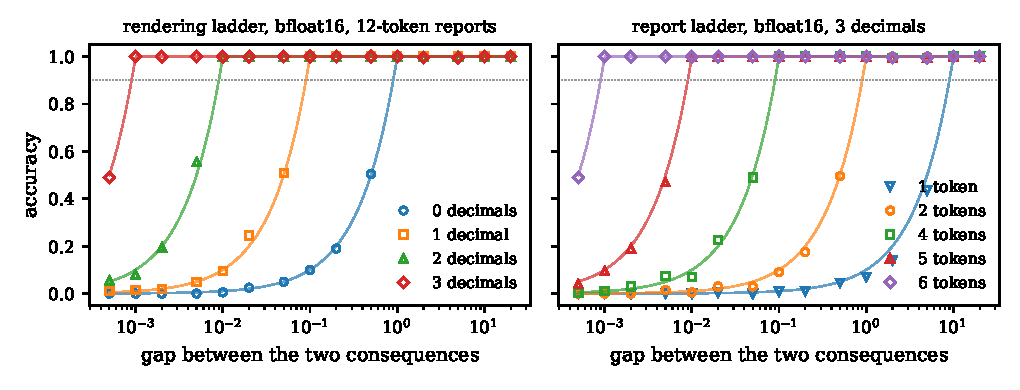
\includegraphics[width=\columnwidth]{figures/accuracy.pdf}
\caption{Accuracy against gap, bfloat16 weights, with the grid-channel law $\min(1,\Delta/h)$ drawn through each cell at the step that was set.
Left, the rendering ladder at full report length.
Right, the report ladder at three decimals.
Every point sits on its line: the accuracy at a gap is the gap divided by the grid step, and the line moves by one decade with each step of the budget.
The dotted line is the 0.9 level of the registered threshold.}
\label{fig:accuracy}
\end{figure}

\begin{figure}[t]
\centering
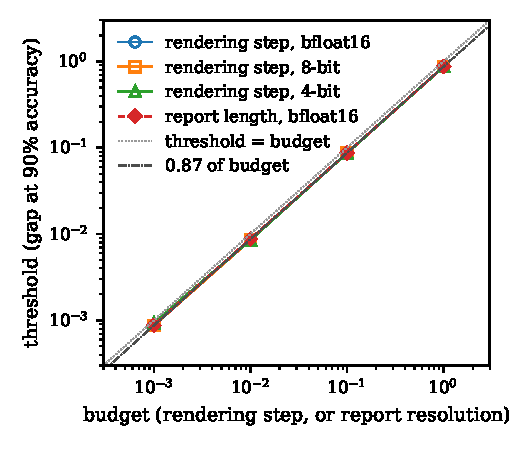
\includegraphics[width=0.56\columnwidth]{figures/thresholds.pdf}
\caption{The registered threshold against the budget that was set, log axes.
Rendering cells at three weight precisions, and the report ladder.
Every point lies on the line at 0.87 of the budget, which is where the registered estimator, log-gap interpolation to the 0.9 level on this ladder, places the threshold of a grid channel.
The three weight precisions coincide.
The fitted steps in Table~\ref{tab:fit} are the quantity to read; this figure shows that the sealed statistic behaved as the proposition says it must.}
\label{fig:thresholds}
\end{figure}

\begin{table}[t]
\centering
\small
\caption{The step fitted from each accuracy curve against the step that was set, with 95 percent bootstrap intervals, and the lapse above resolution.
Rendering cells at 12-token reports; report cells at 3 decimals and bfloat16.
The registered threshold at the 0.9 level is shown for the record.
Every graded interval contains the set step. The one-token cell is reported and not graded.}
\label{tab:fit}
\begin{tabular}{llrrrrr}
\toprule
Cell & weights & set $h$ & $\hat h$ & interval & $\hat h/h$ & lapse $\hat\lambda$ \\
\midrule
0 decimals & bf16, 8-bit, 4-bit & 1 & 0.998 & [0.89, 1.14] & 1.00 & 0.000 \\
1 decimal & bf16, 8-bit, 4-bit & 0.1 & 0.0957 & [0.086, 0.109] & 0.96 & 0.000 \\
2 decimals & bf16, 8-bit, 4-bit & 0.01 & 0.00924 & [0.0083, 0.0104] & 0.92 & 0.000 \\
3 decimals & bf16 & 0.001 & 0.00102 & [0.00089, 0.00119] & 1.02 & 0.001 \\
3 decimals & 8-bit & 0.001 & 0.00102 & [0.00089, 0.00118] & 1.02 & 0.001 \\
3 decimals & 4-bit & 0.001 & 0.00099 & [0.00087, 0.00115] & 0.99 & 0.031 [0.024, 0.038] \\
\midrule
1 token & bf16 & 10 & 11.9 & [10.4, 13.8] & 1.19 & 0.000 \\
2 tokens & bf16 & 1 & 1.03 & [0.92, 1.17] & 1.03 & 0.000 \\
3 tokens & bf16 & 1 & 1.03 & [0.92, 1.17] & 1.03 & 0.002 \\
4 tokens & bf16 & 0.1 & 0.100 & [0.090, 0.113] & 1.00 & 0.001 \\
5 tokens & bf16 & 0.01 & 0.0106 & [0.0094, 0.0122] & 1.06 & 0.001 \\
6 tokens & bf16 & 0.001 & 0.00102 & [0.00089, 0.00119] & 1.02 & 0.001 \\
\bottomrule
\end{tabular}
\end{table}

The sealed verdict is a pass on P1, P1b, P2 and P3.
Figure~\ref{fig:accuracy} shows the accuracy curves, Table~\ref{tab:fit} the fitted steps, and Figure~\ref{fig:thresholds} the registered thresholds.
No report was unparsable in any cell.
The registered thresholds, at bfloat16, were 0.869, 0.0868, 0.00856, and 0.00087 at 0 to 3 decimals and 8.85, 0.872, 0.872, 0.0873, 0.00877, and 0.00087 at 1 to 6 tokens, each with a bootstrap interval of width below three percent of its value, and the 8-bit and 4-bit thresholds equal the bfloat16 values to the digits shown except at three decimals under 4-bit weights, 0.00093, a ratio of 1.06 inside the registered tolerance of 1.5.

\paragraph{The accuracy curve is the grid-channel law.}
In every cell the accuracy at a gap below the set step equals the gap divided by the step, and above the step it is one, to within the binomial noise of 200 pairs.
The largest deviation from $\min(1,\Delta/h)$ at any ladder point in any graded cell is 0.055, at a point where the law predicts 0.5 and the standard error is 0.035.
The step fitted from the curve is within eight percent of the step that was set in every graded cell, and every interval contains the set step.
That is the content of Figure~\ref{fig:accuracy}: the curves are one line, $\Delta/h$, drawn at four values of $h$ on the left and five on the right.

\paragraph{Rendering and report length are the same budget.}
A grid on what the judge reads and a grid on what it writes produce the same accuracy curve at the same step.
At three decimals and two tokens the fitted step is 1.03 against 1; at one decimal and full report it is 0.096 against 0.1; at two decimals and five tokens the two fitted steps are 0.0092 and 0.0106 against 0.01.
Two and three tokens give the same step because the third character is the decimal point, and six and twelve tokens give the same step because the three-decimal rendering is the floor.
This is the length budget of Definition~\ref{def:object} on both sides of the evaluator: the symbols the judge is given and the symbols it may spend set its resolution, and nothing between them does.

\paragraph{Weight precision changes reliability and not resolution.}
At 8-bit weights every accuracy curve equals its bfloat16 curve to the digits shown.
At 4-bit weights the curves at 0, 1, and 2 decimals equal the bfloat16 curves, and at three decimals the fitted step is 0.00099 against 0.00102 at bfloat16, an interval of $[0.00087,0.00115]$ containing the set step, while the accuracy above resolution falls from 0.99 to 1.00 to a plateau of 0.95 to 0.98.
The two-parameter law reads this as a step unchanged and a lapse of 0.031, interval $[0.024,0.038]$, where the bfloat16 and 8-bit judges have a lapse of 0.001.
The registration named the weight ladder as the place where the threshold prediction could fail, and it did not.
What the weights did move is a second property, the judge's reliability once a difference is resolved.
On this task, then, a judge has two numbers and not one: a resolution, set by the symbol grid on either side of it, and a reliability above that resolution, which its weight precision can lower without moving the resolution.

\paragraph{Well-separated pairs keep their order, on one gap.}
The largest registered threshold in any cell is 8.85, in the ungraded one-token cell, so the only ladder gap at least twice that is 20, and P3 as registered is a single-gap test.
At gap 20 the worst accuracy over all eighteen cells is 0.985.
A budget change enlarged the threshold by four orders of magnitude and reordered nothing at that gap.
A registration with gaps beyond 20, and with P3 defined on the largest graded threshold, is the natural next gate and is listed in Section~\ref{sec:scope}.

\subsection{Identification on synthetic evaluators}
\label{sec:gates}

Theorem~\ref{thm:repr}(c) says what choices can recover, and the gate that tests it uses the whole-space case that is machine-checked.
Forty evaluators per cell, in two to four dimensions with random metrics including singular ones, were given batteries of consequences of increasing size, and the feasibility program of Theorem~\ref{thm:repr}(a) with a margin was solved from their weak orders alone.
Errors were scored against the chance level of guesses from the evaluator prior.
In all twelve cells on a fresh seed, under a sealed registration, the metric and the ideal's range component were recovered at 64 consequences above the dimension, to a few percent of chance, with the error falling at every step as the battery grew, while at or below the design bound, off the span of a battery confined to a subspace, and in the kernel of a singular metric, nothing was recovered.
A semiorder that withholds the fifth of pairs closest in distance identified more slowly, to between 5 and 25 percent of chance at the same battery.
Further sealed gates, a hull law on a public survey that held as a population tendency, the same law on natural decisions where the violation rate fell with the rank at which consequences were read, as registered, and a shared-representation bound on attention heads that returned indeterminate, are reported in Appendix~\ref{app:gates} at the size of their verdicts.

\section{Verification of the exact distributions}
\label{app:verify}

The read-outs that use samples do not generate them.
They draw from a score distribution computed exactly, which removes one full pass of the prompt per sample.
This appendix reports the checks that the computed distribution is the one the judge samples from.
All were run before the registration was sealed, on the 7B judge at bfloat16 unless stated, and the records are in the supplementary material.

\paragraph{Single-token scales.}
On the 1 to 5 and 0 to 9 scales a score is one token, and the distribution is the first-token distribution restricted to the codebook.
On a block of 42 worksheets no report was unparsable on any scale and all first-token mass fell on the codebook.
Real samples at temperature one were compared with the recorded distribution on six worksheets of the 0 to 9 scale, at 0, 4, 8, 12, 16 and 20 errors, with 256 draws each.
The statistic is the total variation distance, and the bar is the 95th percentile of that distance under multinomial sampling from the recorded distribution.
Five worksheets fell inside the bar.
The worksheet with 16 errors did not, at 0.105 against 0.073.
Two follow-ups placed the miss as chance.
The distribution did not depend on batch shape: computed alone, in 32 copies, and inside a padded batch of mixed prompts, it was identical, which rules out bfloat16 batch numerics.
Redrawn with 2{,}048 samples the same worksheet sat at 0.015 against a bar of 0.026 ($p=0.36$), and the worksheet with 12 errors at 0.014 against 0.027 ($p=0.59$).

\paragraph{The digit tree.}
On the 0 to 100 scale a score takes up to three digit tokens.
One pass gives the first digit.
Every digit prefix with probability above $10^{-5}$ is extended by one cached single-token step that gives each next digit and the probability of stopping, with the model's repetition penalty applied as sampling applies it.
The pruned mass, the mass on values outside the scale, and the mass on a first token that is not a digit are recorded for every worksheet.
On six worksheets, 1{,}024 real samples each matched the tree's distribution within multinomial noise in all six, with $p$ from 0.21 to 0.95, no unparsable or out-of-range draw, and at most $6.2\times10^{-5}$ of the mass pruned.
Over the 42-worksheet block the pruned mass was at most $1.2\times10^{-4}$, no mass fell outside the scale, and the first token was always a digit.
Recomputing the tree's 37 largest probabilities by one uncached forward pass each gave relative differences of up to 24 percent.
That is one bfloat16 rounding step in the logits, about 0.125 at the logit sizes seen here, between the cached decoding path that sampling uses and an uncached full pass.
A judge's score distribution is therefore defined only up to one bfloat16 step in its logits, depending on the kernel path, and the tree reproduces the path that sampling takes, which is what the agreement with real samples shows.
The tree scores a worksheet in 1.16 seconds, against 4.5 for generating eight samples.

\paragraph{The chunked tree for the 14B judge.}
The 14B judge ran out of memory at the second digit of the tree, because every live two-digit prefix carried its own copy of the prompt's cache beside 27.5 GiB of weights on a 31.7 GiB card.
For that judge alone the tree runs the same single-token step on at most eight prefixes at a time and keeps the cache only of prefixes that have children.
Every other judge uses the whole-frontier tree unchanged.
On 22 worksheets the 7B judge's chunked and whole-frontier trees differed by at most $5.2\times10^{-5}$ in any probability, which is batch composition in bfloat16.
The 14B judge's chunked tree matched brute force on eight scores to a relative difference of at most 0.21, the largest on a score of probability 0.07, against 0.24 for the 7B judge's tree.
It scores a worksheet in 3.7 seconds at a peak of 29.5 GiB.


\section{Proofs}
\label{app:proofs}

\begin{proof}[Proof of Theorem~\ref{thm:dist}]
(a) Equality almost everywhere is an equivalence relation.
(b) The relation is equality of a function of $a$, hence an equivalence, and $C(a,x)=C(b,x)$ implies equality of the retained projections, so each $\sim_{k}$ class contains the $\sim$ classes of its members.
(c) Reflexivity and symmetry are immediate.
If three such points exist then $r_{1}\approx_{\varepsilon}r_{2}$ and $r_{2}\approx_{\varepsilon}r_{3}$ but not $r_{1}\approx_{\varepsilon}r_{3}$.
If none exist, take $a\approx_{\varepsilon}b\approx_{\varepsilon}c$ with values $r_{a},r_{b},r_{c}$.
If $r_{a}\le r_{b}\le r_{c}$ or the reverse, the absence of such a triple gives $|r_{a}-r_{c}|\le\varepsilon$, and in every other ordering $|r_{a}-r_{c}|\le\max(|r_{a}-r_{b}|,|r_{b}-r_{c}|)\le\varepsilon$.
\end{proof}

\begin{proof}[Proof of Theorem~\ref{thm:pref}]
(a) A relation defined by comparing a real function is complete and transitive, and the function represents it. Uniqueness up to monotone transformation is the standard ordinal uniqueness.
(b) A relation defined by $u(a)>u(b)+\varepsilon$ with fixed $\varepsilon>0$ is irreflexive and satisfies the two semiorder axioms.
If $a\succ b$ and $c\succ e$, then $u(a)>u(b)+\varepsilon$ and $u(c)>u(e)+\varepsilon$, so either $u(a)>u(e)+\varepsilon$ or $u(c)>u(b)+\varepsilon$, since if both failed we would have $u(a)\le u(e)+\varepsilon<u(c)$ and $u(c)\le u(b)+\varepsilon<u(a)$, a contradiction.
If $a\succ b\succ c$ and $e$ is any action, then $u(a)>u(c)+2\varepsilon$, so either $u(a)>u(e)+\varepsilon$ or $u(e)\ge u(a)-\varepsilon>u(c)+\varepsilon$.
This is the easy direction of the Scott and Suppes representation of semiorders, and the representation is by construction.
(c) The semiorder is a weak order exactly when indifference is transitive, which is Theorem~\ref{thm:dist}(c), and for finite $A$ the condition holds for all sufficiently small $\varepsilon$.
\end{proof}

\begin{proof}[Proof of Theorem~\ref{thm:repr}]
(a) Given $(G,t)$, put $M=[\,I\;\;-t\,]$, an $m\times(m+1)$ matrix, and $W=M^{\top}GM$.
Then $W$ is positive semidefinite and $Q_{W}(y)=(y-t)^{\top}G(y-t)=q(y)$, so the order constraints hold for $W$.
Conversely let $W$ be positive semidefinite with blocks $G$, $b/2$, $b^{\top}/2$, $\gamma$, so that $Q_{W}(y)=y^{\top}Gy+b^{\top}y+\gamma$.
Then $G$ is positive semidefinite, and $b$ lies in the range of $G$: if $Gz=0$ then $(z,s)W(z,s)^{\top}=s\,b^{\top}z+\gamma s^{2}\ge0$ for every real $s$, which forces $b^{\top}z=0$.
Choose $t$ with $Gt=-b/2$.
Then $Q_{W}(y)=(y-t)^{\top}G(y-t)+\gamma-t^{\top}Gt$ differs from $q$ by a constant, so $(G,t)$ orders $A$ as $Q_{W}$ does.
The order constraints are linear in the entries of $W$ for fixed consequences, and the cone is convex.
(b) $q$ is convex because $G$ is positive semidefinite.
If $y_{a}=\sum_{s}\lambda_{s}y_{s}$ with $\lambda_{s}\ge0$ summing to one, then $q(y_{a})\le\sum_{s}\lambda_{s}q(y_{s})\le\max_{s}q(y_{s})$, so $a\succsim s^{*}$ for a maximizer $s^{*}$.
The argument used only convexity.
(c) Same weak order on $U$ means $q_{2}=\varphi\circ q_{1}$ on $U$ for a strictly increasing $\varphi$ on $q_{1}(U)$, an interval because $U$ is connected and $q_{1}$ is continuous.

\emph{Metric.}
Fix $y\in U$ and a direction $v$ with $v^{\top}G_{1}v>0$, and write $g_{i}=v^{\top}G_{i}v$, $\ell_{i}=v^{\top}G_{i}(y-t_{i})$.
Along $y+sv$, $q_{1}=q_{1}(y)+2\ell_{1}s+g_{1}s^{2}$ and $q_{2}=q_{2}(y)+2\ell_{2}s+g_{2}s^{2}$, both quadratics in $s$, and $q_{2}=\varphi(q_{1})$ on an interval of $s$ around $0$.
Two quadratics in $s$ related by a strictly increasing map on an interval have the same critical point if the interval contains it, and in general the level sets of $q_{1}$ along the segment, which are pairs $\{s,s'\}$ symmetric about $s^{*}_{1}=-\ell_{1}/g_{1}$, must be level sets of $q_{2}$.
If the segment contains two distinct such pairs, $q_{2}$ is symmetric about the same point, so $s^{*}_{2}=s^{*}_{1}$ and $\varphi$ is affine on the traced interval with slope $g_{2}/g_{1}$.
When $\operatorname{rank}G_{1}\ge2$ such a segment exists through every $y\in U$: choose $v$ with $v^{\top}G_{1}v>0$ and $v^{\top}G_{1}(y-t_{1})=0$, which exists because a positive semidefinite form of rank at least two does not vanish on the hyperplane $\{v:v^{\top}G_{1}(y-t_{1})=0\}$, and then $s^{*}_{1}=0$ is interior to the segment.
When $\operatorname{rank}G_{1}=1$, write $G_{1}=g\,ww^{\top}$; the level sets of $q_{1}$ in $U$ are pieces of the hyperplanes $w^{\top}y=$ const, $q_{2}$ is constant on each, so $q_{2}$ restricted to $U$ is a function of $w^{\top}y$ alone, hence a quadratic in $w^{\top}y$, and its quadratic part is $g'\,ww^{\top}$ with $g'>0$ because $q_{2}$ is nonconstant on $U$.
In both cases $G_{2}=\lambda G_{1}$ with $\lambda>0$: in the rank-one case directly, and in the higher-rank case because $\varphi$ is affine with the same slope $\lambda$ on overlapping intervals along every chain of segments through the connected set $U$, so $q_{2}=\lambda q_{1}+\mu$ on the open set $U$, two polynomials that agree on an open set agree identically, and the quadratic parts match.

\emph{Ideal.}
In the case $\operatorname{rank}G_{1}\ge2$ the identity $q_{2}=\lambda q_{1}+\mu$ also matches linear parts, $G_{2}t_{2}=\lambda G_{1}t_{1}$, which with $G_{2}=\lambda G_{1}$ is $G_{1}(t_{2}-t_{1})=0$.
In the case that $U$ contains a minimizer $y^{*}$ of $q_{1}$, so $G_{1}(y^{*}-t_{1})=0$, every segment through $y^{*}$ in a direction with $v^{\top}G_{1}v>0$ has $s^{*}_{1}=0$ interior, and the argument above gives $v^{\top}G_{2}(y^{*}-t_{2})=0$ for every such $v$, hence for a spanning set of the range of $G_{1}$, and with $G_{2}=\lambda G_{1}$ this is $G_{1}(y^{*}-t_{2})=0$ and so $G_{1}(t_{2}-t_{1})=0$.
When neither hypothesis holds the ideal need not be identified, as the one-dimensional example after the theorem shows.
\end{proof}

\begin{proof}[Resolution reversal]
Take $\Y=\R^{2}$, $G=I$, $t=0$, $X$ a point, and a workload whose consequence second moment has top eigenvector $e_{1}$, for example $\operatorname{diag}(4,1)$.
Let $C(a)=(1,0)$ and $C(b)=(0.9,2)$.
Then $d_{1}(a)=1$, $d_{1}(b)=0.9$, $d_{2}(a)=1$, and $d_{2}(b)=\sqrt{0.81+4}=2.19$, so $b\succ a$ at rank cap 1 and $a\succ b$ at rank cap 2.
A function representing both would satisfy $u(b)>u(a)$ and $u(a)>u(b)$.
\end{proof}

\section{Tokenization and parsing of reports}
\label{app:tokens}

The report-length ladder rests on the claim that the judge emits one character per generated token for the digits and the decimal point.
Table~\ref{tab:tokens} shows the token identifiers the recorded tokenizer revision assigns to representative reports.
Each digit and the decimal point is a single token, so a report limited to $k$ tokens is the decimal expansion of the judge's answer truncated to $k$ characters.
A report is parsed as the first number in the decoded string, a trailing decimal point is dropped, and a string with no number counts as unparsable and as indifference.
No report was unparsable in any cell of the run.
The probes at full report length, whose raw generations are in the record, show the judge answering with exactly three decimals and rounding the last, for example a true distance of 11.6876 reported as 11.688 and 10.2039 as 10.204.
The record does not hold per-pair generations for the run or the count of reports that stopped before the budget, which a future gate will log under the programme's rule that every stage persists what it saw.

\begin{table}[h]
\centering
\small
\caption{Token identifiers for representative reports under the recorded tokenizer revision. One character per token.}
\label{tab:tokens}
\begin{tabular}{lll}
\toprule
report & token identifiers & decoded tokens \\
\midrule
\texttt{10} & 16, 15 & 1, 0 \\
\texttt{10.} & 16, 15, 13 & 1, 0, . \\
\texttt{10.1} & 16, 15, 13, 16 & 1, 0, ., 1 \\
\texttt{10.12} & 16, 15, 13, 16, 17 & 1, 0, ., 1, 2 \\
\texttt{10.123} & 16, 15, 13, 16, 17, 18 & 1, 0, ., 1, 2, 3 \\
\texttt{27.375} & 17, 22, 13, 18, 22, 20 & 2, 7, ., 3, 7, 5 \\
\texttt{0.001} & 15, 13, 15, 15, 16 & 0, ., 0, 0, 1 \\
\bottomrule
\end{tabular}
\end{table}

\section{Two further sealed gates}
\label{app:gates}

\paragraph{Hull law on a public survey, pass as a tendency.}
Theorem~\ref{thm:repr}(b) needs only a known consequence map and observed choices.
In the 1972 American National Election Study respondents placed candidates and parties on seven-point issue scales and rated them on feeling thermometers, so the consequence of an object is its position on a registered pair of scales and the choice is the rating.
On the registered pair, 489 of 557 respondents had a menu in which the law could bind, and 246 of them, 50.3 percent, violated it at least once, against 66.4 percent when each respondent's ratings are shuffled among that respondent's own objects, with none of 200 shuffles reaching the observed rate.
Five other pairs of scales gave the same ordering, observed rates of 54 to 63 percent against shuffled rates of 67 to 74 percent.
The rates sit well below the geometric base rate of violation and well above zero.
The registration recorded both halves, that the law holds as a population tendency and that about half of the respondents violate it.
The second half needs a qualification found after that gate was graded.
A pair of scales is a rank-two reading of whatever space a respondent evaluates in.
A convex combination survives any linear map, so a point inside a hull stays inside under projection while a point outside can fall inside.
Reading fewer coordinates can therefore add violations and cannot remove them, and the observed rate bounds the rate in the respondent's own space from above rather than estimating it.
That omitted attributes can make rational choice fail a revealed-preference test is established for characteristics models \citep{blow2008revealed}, and the next gate measures the size of the effect.

\paragraph{The same law on natural decisions, read at increasing rank, pass.}
The cap of Theorem~\ref{thm:dist}(b) is a cap on the rank at which consequences are read, and two sealed gates apply it from the analyst's side to choices nobody elicited.
In ten regular seasons of professional football play calls, 303{,}414 decisions, the consequence of a call is a five-coordinate vector estimated from outcomes and pooled over every team, and a team's ranking of calls in a game state is its choice share.
With four calls a menu can bind only on a plane, because four points in general position never place one inside the hull of the others above two dimensions.
On the registered pair of coordinates 8 of 402 testable units violated the law, 2.0 percent against 22.9 percent shuffled, with none of 200 shuffles reaching the observed rate, and on one replication pair the law was violated above chance, 30.0 against 22.1 percent.
That gate graded indeterminate under its own sensitivity clause.
A follow-on gate with thirteen calls registered, before any rate in that menu had been computed, that the violation rate would not rise as more of the five coordinates are read.
Over every graded subset the mean rate was 0.914 at two coordinates, 0.444 at three, and 0.139 at four, and all 26 subsets sat below their shuffled rate, including the pair that had been violated above chance.
Perturbing each consequence by its own standard error moved that pair's rate by 0.089 against a margin of 0.079 over its null, and moved the registered pair's by 0.006 against a margin of 0.209.
Reading more of the consequence space lowers the rate, which is the ordering Section~\ref{sec:budgets} predicts for a judge's read-outs, in a world with no language model in it.
A second arm, which tried to recover a metric from pooled choices, recovered none.
One metric and one ideal served about eight game states and a stratum held 189, so that arm is a miss of the measurement and is reported as one.

\paragraph{Shared-representation regret, indeterminate.}
Let $N$ evaluators share a representation space $\R^{d}$ with constant pullbacks $P_{1},\dots,P_{N}$ and a common isotropic source of second moment $\sigma^{2}I$, and let a shared representation at budget $k$ be an orthogonal projector $\Pi$ of rank $k$.
Evaluator $i$'s regret from $\Pi$ is $r_{i}(\Pi)=\sigma^{2}(\sum_{j\le k}\lambda_{j}(P_{i})-\tr(\Pi P_{i}))\ge0$.
A shared representation with zero regret for every evaluator exists if and only if there is a $k$-dimensional subspace that is a top-$k$ eigenspace of every $P_{i}$, and for weights $w_{i}>0$ the least weighted total regret is attained by a top-$k$ eigenspace of $\bar P=\sum_{i}w_{i}P_{i}$, strictly positive exactly when no common eigenspace exists.
Both statements are Ky Fan's maximum principle \citep{fan1949}, and the regret formula is the second-order expansion of the loss under a rank-$k$ code.
The gate took the three query heads of a grouped-query attention group in a language model as evaluators of one key cache, with shared codes of rank 2, 4, and 8 in 128 dimensions.
At those ranks the measured attention loss was 20 to 330 times the second-order prediction, so the regret formula and its bound could not be tested and the verdict is indeterminate.
The ordering claim survived on the measured losses alone: the leading eigenspace of the summed geometries beat every random code and the key-covariance code in 32 of 32 cases, while a head's own leading eigenspace was the best code for that head in fewer than half the cases.
A second sealed run perturbed one key at a time by a small isotropic error in the discarded subspace, where the measured loss matched the second-order prediction at the median, a ratio of 1.02 to 1.05, while 64 draws per cell left a 20 percent scatter that missed the registered per-triple bar, so that verdict is indeterminate as well.
The registration of the first run also compared a one-key prediction to an all-keys measurement, a defect recorded rather than repaired after the fact.

\section{Per-cell accuracy}
\label{app:cells}

Table~\ref{tab:cells} gives the accuracy at every ladder gap in every cell of the run, from which the registered thresholds and the fits of Table~\ref{tab:fit} were computed.

\begin{table}[h]
\centering
\scriptsize
\caption{Accuracy by gap for all eighteen cells. Columns are the gap ladder. Cells are weight precision, decimals, report tokens.}
\label{tab:cells}
\setlength{\tabcolsep}{3pt}
\begin{tabular}{lrrrrrrrrrrrrrrr}
\toprule
cell & .0005 & .001 & .002 & .005 & .01 & .02 & .05 & .1 & .2 & .5 & 1 & 2 & 5 & 10 & 20 \\
\midrule
bf16, 0, 12 & 0.00 & 0.00 & 0.00 & 0.00 & 0.01 & 0.03 & 0.05 & 0.10 & 0.19 & 0.51 & 1.00 & 1.00 & 1.00 & 1.00 & 1.00 \\
bf16, 1, 12 & 0.01 & 0.01 & 0.02 & 0.05 & 0.10 & 0.24 & 0.51 & 1.00 & 1.00 & 1.00 & 1.00 & 1.00 & 1.00 & 1.00 & 1.00 \\
bf16, 2, 12 & 0.06 & 0.08 & 0.20 & 0.56 & 1.00 & 1.00 & 1.00 & 1.00 & 1.00 & 1.00 & 1.00 & 1.00 & 1.00 & 1.00 & 1.00 \\
bf16, 3, 12 & 0.49 & 1.00 & 1.00 & 1.00 & 1.00 & 1.00 & 1.00 & 1.00 & 1.00 & 1.00 & 1.00 & 0.99 & 0.99 & 1.00 & 1.00 \\
bf16, 3, 1 & 0.00 & 0.00 & 0.00 & 0.00 & 0.00 & 0.01 & 0.00 & 0.01 & 0.01 & 0.04 & 0.07 & 0.14 & 0.43 & 1.00 & 1.00 \\
bf16, 3, 2 & 0.00 & 0.00 & 0.00 & 0.01 & 0.01 & 0.03 & 0.03 & 0.09 & 0.17 & 0.49 & 1.00 & 1.00 & 1.00 & 1.00 & 1.00 \\
bf16, 3, 3 & 0.00 & 0.00 & 0.01 & 0.02 & 0.01 & 0.03 & 0.03 & 0.09 & 0.17 & 0.49 & 1.00 & 0.99 & 0.99 & 1.00 & 1.00 \\
bf16, 3, 4 & 0.01 & 0.01 & 0.03 & 0.07 & 0.07 & 0.23 & 0.49 & 1.00 & 1.00 & 1.00 & 1.00 & 0.99 & 0.99 & 1.00 & 1.00 \\
bf16, 3, 5 & 0.04 & 0.10 & 0.19 & 0.47 & 1.00 & 1.00 & 1.00 & 1.00 & 1.00 & 1.00 & 1.00 & 0.99 & 0.99 & 1.00 & 1.00 \\
bf16, 3, 6 & 0.49 & 1.00 & 1.00 & 1.00 & 1.00 & 1.00 & 1.00 & 1.00 & 1.00 & 1.00 & 1.00 & 0.99 & 0.99 & 1.00 & 1.00 \\
8-bit, 0, 12 & 0.00 & 0.00 & 0.00 & 0.00 & 0.01 & 0.03 & 0.05 & 0.10 & 0.19 & 0.51 & 1.00 & 1.00 & 1.00 & 1.00 & 1.00 \\
8-bit, 1, 12 & 0.01 & 0.01 & 0.02 & 0.05 & 0.10 & 0.24 & 0.51 & 1.00 & 1.00 & 1.00 & 1.00 & 1.00 & 1.00 & 1.00 & 1.00 \\
8-bit, 2, 12 & 0.06 & 0.08 & 0.20 & 0.56 & 1.00 & 1.00 & 1.00 & 1.00 & 1.00 & 1.00 & 1.00 & 1.00 & 1.00 & 1.00 & 1.00 \\
8-bit, 3, 12 & 0.49 & 1.00 & 1.00 & 1.00 & 1.00 & 1.00 & 1.00 & 1.00 & 1.00 & 1.00 & 1.00 & 0.99 & 0.99 & 1.00 & 1.00 \\
4-bit, 0, 12 & 0.00 & 0.00 & 0.00 & 0.00 & 0.01 & 0.03 & 0.05 & 0.10 & 0.19 & 0.51 & 1.00 & 1.00 & 1.00 & 1.00 & 1.00 \\
4-bit, 1, 12 & 0.01 & 0.01 & 0.02 & 0.05 & 0.10 & 0.24 & 0.51 & 1.00 & 1.00 & 1.00 & 1.00 & 1.00 & 1.00 & 1.00 & 1.00 \\
4-bit, 2, 12 & 0.06 & 0.08 & 0.20 & 0.56 & 1.00 & 1.00 & 1.00 & 1.00 & 1.00 & 1.00 & 1.00 & 1.00 & 1.00 & 1.00 & 1.00 \\
4-bit, 3, 12 & 0.49 & 0.95 & 0.97 & 0.97 & 0.97 & 0.95 & 0.96 & 0.96 & 0.98 & 0.96 & 0.95 & 0.98 & 0.98 & 0.97 & 0.98 \\
\bottomrule
\end{tabular}
\end{table}

\end{document}
